\documentclass[10pt,a4paper,notitlepage,oneside,twocolumn]{abst_jsarticle}
% notitlepage : \titlepage は独立しない
% oneside : 奇数・偶数ページは同じデザイン
% twocolumn : 2段組
% \setlength{\textwidth}{\fullwidth}
% 本文領域はページ一杯で, 傍注の幅を取らない

\usepackage[dvipdfmx]{graphicx, color}
% \usepackage{amsmath}
\usepackage{amsmath,amssymb}
\usepackage{comment}

\usepackage{url}
\usepackage{bm}
\usepackage{here}
\usepackage{algorithm}
\usepackage{algpseudocode}
\usepackage{hhline} 
\usepackage[hang,small,bf]{caption}
\usepackage[subrefformat=parens]{subcaption}
% \usepackage{tabularx}
% \usepackage[dvipdfm]{graphicx}
%\numberwithin{equation}{section}

\usepackage[hmargin=2truecm, textheight= 78zw]{geometry}
\columnsep=\dimexpr \textwidth - 50zw \relax

%%\unitlength=1pt
%%\renewcommand{\baselinestretch}{0.8}

\title{
{\bf 高解像度の煙シミュレーションの高速化}
}

\author{\begin{center}
{\large {\bf 23N8100018BC 須之内 俊樹}}\\
{\large {\bf 情報工学専攻 形状情報処理研究室}}\\
{\large {\bf 2023年7月}}
\end{center}}

\date{}
\pagestyle{empty}

\begin{document}

\maketitle
%%%%%%%%%%%%%%%%%%%%%%%%%%%%%%
\section{流体シミュレーション} \label{sec:intro}
流体の運動を記述する数理モデルの近似解を求めることを,流体シミュレーションという.計算機を使った流体力学を特別に,数値流体力学 (CFD: Computational Fluid Dynamics) と呼ぶ.CFDは計算機を用いない実験で得ることが困難な,流れ場全体の詳細な情報を得ることができる.CGの分野では流体の動きを忠実に再現することよりも,それらしい流体の運動を計算負荷を抑えて計算することが重視されている.流体の種類や運動によって条件を設けることで,よりそれらしい動きをシミュレーションすることができる.

次の2つの式を合わせてナビエ・ストークス方程式と呼び,これは流体力学の支配方程式である.非線形二階微分方程式となっており,代数的に一般解を求める事ができない.
\begin{equation}\label{eq:Navie}
\frac{\partial}{\partial t}\bm{u} = - (\bm{u} \boldsymbol{\cdot}\nabla) \bm{u} - \frac{1}{\rho}\nabla p + \nu\nabla^2\bm{u} + \bm{f}
\end{equation}
%\begin{equation}\label{eq:uncompressed}
$$\nabla\boldsymbol{\cdot}\bm{u} = 0$$
%\end{equation}
ここで,$t$は時刻,$\varDelta x,\varDelta t$はそれぞれ,離散化する計算格子の格子幅,次の時刻までの時間幅,$\bm{u},p$は位置$\bm{x}$,時刻$t$での流体の速度ベクトル場,圧力のスカラー場,$\rho,\nu$はそれぞれ,流体の密度,流体の粘性,$\bm{f}$ 位置$\bm{x}$,時刻$t$での流体にかかる外力ベクトル,$\nabla$は空間微分演算子ナブラを表している.

数値流体力学ではシミュレーションする空間や時間を離散化して近似解を求める.空間の離散化は,各辺が空間の座標軸に並行な計算格子を用いて空間を分割し計算格子上に物理量を配置する格子法と,流体を粒子で表現し粒子上に物理量を配置する粒子法がある.ある時刻で空間の物理量の分布を計算した後,時刻を時間の刻み幅分進めて次の時刻の計算をすることを繰り返してシミュレーションを行う.

式\ref{eq:Navie}の右辺の第一項を移流項,第二項を圧力項,第三項を粘性項,第四項を外力項とよぶ.移流項は非線形項であり,その他は線形項である.
格子法における移流項の計算方法として,次の式で表されるStamのSemi-Lagrangian法\cite{semi-Lagrangian}がある.
Semi-Lagrangian法は, 位置$\bm{x}$,時刻$t$での流体の速度ベクトルを${u}_{t+\Delta t}(\bm{x})$とすると,以下のように表せる.
%\begin{equation}\label{eq:semi-Lagrangian}
$$\bm{u}_{t+\Delta t}(\bm{x}) = \bm{u}_t(\bm{x}-\bm{u}_t(\bm{x}))$$
%\end{equation}
陽解法だと$\Delta t$大きくとると計算が安定しないが,Semi-Lagrangian法は陰解法であり,$\Delta t$を大きく取ることができる.Semi-Lagrangian法は線形補間で容易に実装でき,CGでは広く用いられている.

圧力項の計算方法にChorinの射影法\cite{projection}がある.この手法は圧力項の計算を二つの段階に分けて計算する.まず仮の速度を$\bm{u}^*$として以下のポアソン方程式を解く.
\begin{equation}\label{eq:colin_p}
\nabla^2 \bm{p} =  \frac{1}{\Delta t}\nabla\boldsymbol{\cdot}\bm{u}^*
\end{equation} 
ノイマン境界条件は$\frac{\partial p}{\partial \bm{n}} = 0$とする.ポアソン方程式は離散化によって線形方程式に帰着できる.シミュレーション領域の分割数を$n$とすると行列は$n \times n$の疎行列になる.ポアソン方程式を解いた後,下記の式を用いて次の時刻の速度を更新する.

%\begin{equation}\label{eq:colin_v}
$$\bm{u}_{t+\Delta t} = \bm{u}^* - \Delta t \nabla \bm{p}$$
%\end{equation} 

格子法では,流体を可視化する際は密度を元にレンダリングを行う.モデルの表面のみのレンダリングをサーフェスレンダリングという.それに対し,モデルの透明度を計算し,内部の構造を表現するレンダリングをボリュームレンダリングという.サーフェスレンダリングの方が計算負荷が小さく,光の反射や屈折などを計算することができるため,液体や固体はサーフェスレンダリングが用いられる.煙や雲,炎などは表面のレンダリングのみではそれらしい表現にならないため,内部の構造を表現するボリュームレンダリングが用いられる.
\section{関連研究}
CGにおける煙のシミュレーション手法に,Fedkiwらの\cite{fedkiw}がある.この手法は前節で述べた\cite{semi-Lagrangian},\cite{projection}のほか,煙の温度による浮力,渦の力,重力などを外力に加えている.ボリュームレンダリングは密度分布をもとに,格子の透明度と輝度を計算して行う.この手法はそれらしい煙のシミュレーションを実現しているが計算負荷が大きく,解像度$40\times40\times40$の粗い格子でも,計算時間は1フレームあたり1秒ほどかかる.計算時間のほとんどは,式\ref{eq:colin_p}のポアソン方程式に使われている.

流体シミュレーションの計算はGPUを用いた並列計算と相性が良く,シミュレーションの高速化を目指す取り組みもある.Ishidaらの手法\cite{GPU}は,煙は液体と比べ境界が曖昧であるという特徴を利用して,離散コサイン変換を用いて物理量を圧縮し,GPUを用いて高速計算をする手法である.計算方法の大部分は\cite{fedkiw}と同じだが,圧縮した物理量の一部分を展開し,展開した範囲内のみで計算をし,再び圧縮することを繰り返す.式\ref{eq:colin_p}の計算においては行列ではなく,いくつかのベクトルを用いて計算できるため,計算負荷が小さくなる.

近年のGPUを用いた煙のシミュレーションでは,解像度は$256\times512\times256$や,$1024\times1024\times1024$など,文献\cite{fedkiw}らの手法とは桁違いに大きいものになっている.解像度が大きくなると,煙の見た目が詳細になるだけでなく,低解像度では離散化によって均されてしまった物理量の分布が計算できるようになる.

%低解像度でも計算することができる,流体の物理量の大まかな分布を低周波成分という.一方,高解像度で計算することができる,流体の詳細な物理量の分布を,高周波成分という.CGでは高速でそれらしいシミュレーションができることを目指しているため,高解像度のシミュレーションであっても,高速化のために低解像度成分が重要視され,高周波成分を計算しないことがある.
\section{数値実験}
%\begin{figure}[h]
%\begin{center}
%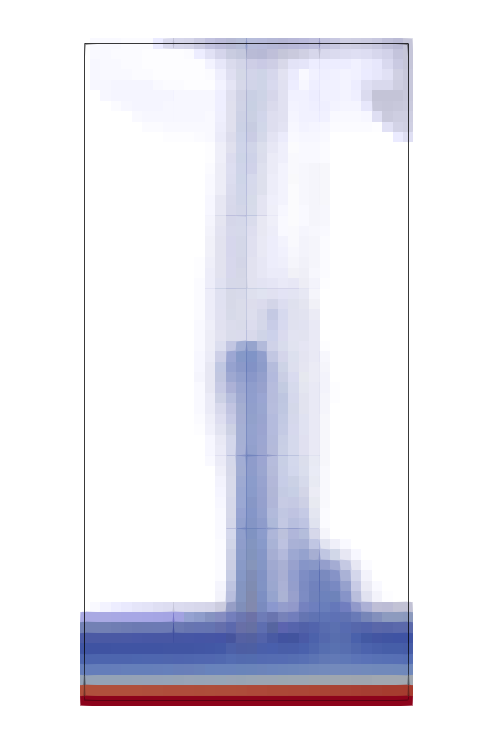
\includegraphics[width=55mm]{center_smoke.png}
%\caption{ParaViewを用いて可視化した様子}
%\label{fig:fig1}
%\end{center}
%\end{figure}

\begin{figure}[h]
\begin{minipage}[t]{0.5\linewidth}
  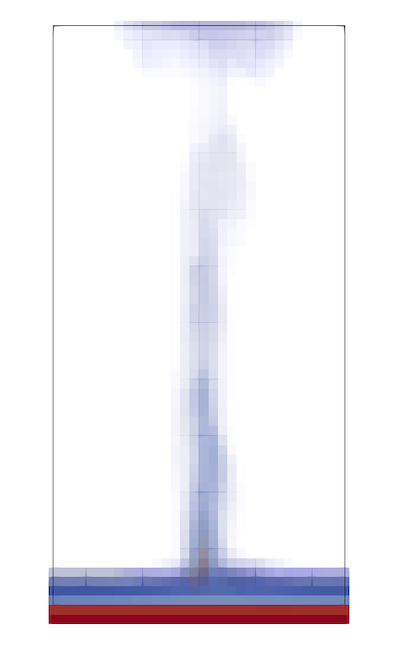
\includegraphics[height=7cm,width=3.5cm]{323264.png}
  \subcaption{}
  \label{fig:fig1}
  \end{minipage}
  \begin{minipage}[t]{0.4\linewidth}
  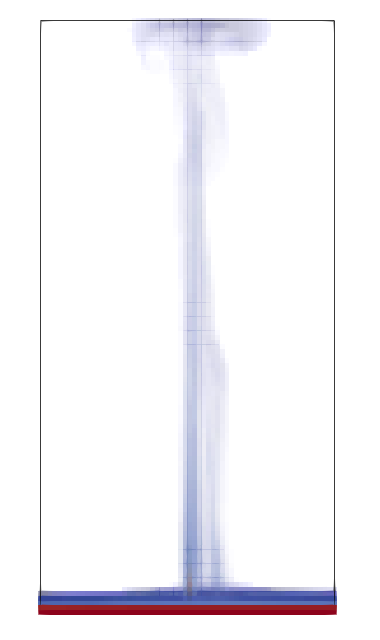
\includegraphics[height=7cm,width=3.5cm]{6464128.png}
  \subcaption{}
  \label{fig:fig2}
  \end{minipage}
\caption{ParaViewを用いて可視化した様子}
\label{fig}
\end{figure}
文献\cite{fedkiw}を参考に格子法を用いた煙のシミュレーション手法を実装した.シミュレーション領域の1つの面に気体を配置し,配置した面の中心に熱源を置いて,煙が上昇する様子をシミュレーションした.図\ref{fig}はシミュレーション結果を,ParaViewを用いて可視化したものである.図\ref{fig:fig1}は解像度$32\times32\times64$のもので,図\ref{fig:fig2}は解像度$64\times64\times128$のものである.密度分布を色と透明度を用いて表示したもので,色は密度が大きいほど赤く,小さいほど青い.透明度は密度に比例し,密度$0$では透明度も$0$である.シミュレーション領域での速度を0にすることで煙が領域の外に出ず,煙が天井にぶつかった後の様子がシミュレーションできる.高い解像度において立ち昇っている煙の分布が分裂している部分が,低い解像度では均されてしまっている.また物理量の分布の変化によって,煙の位置も少し異なっている.
\section{今後の研究計画}
実装した手法は,パラメータの設定によって圧力項計算の結果が収束しない.また,速度が大きくなりすぎてsemi-Lagrangian法では質量保存が成り立たないことがある.計算の安定性は補間方法や,使用する微分スキームによって異なるほか,semi-Lagrangian法において質量保存の式を用いるなどの方法が考えられる.微分スキームの計算の安定性や,semi-Lagrangian法について調査を進め,幅広いパラメータ設定に対応したシミュレーションの実装を目指す.

また,煙の解像度$256\times512\times256$や,$1024\times1024\times1024$などの高解像度の高速なシミュレーション手法について理解を深めるため,文献\cite{GPU}を参考に,離散コサイン変換を利用した展開圧縮手法を実装する.他の高解像度のシミュレーション手法についての論文を参考に,高解像度のシミュレーション手法の高速化手法を模索する.
% 参考文献
\begin{thebibliography}{99}

\bibitem{fedkiw}
R. Fedkiew, J. stam, H. Jensen. Visual simulation of smoke. In \textit{Proceedings of the 28th Annual Conference on Computer Graphics and Interactive Techniques}, SIGGRAPH ’01, pp. 15--22, 2001.

\bibitem{semi-Lagrangian}
J. Stam. Stable fluids. In \textit{Proceedings of the 26th Annual Conference on Computer Graphics and Interactive Techniques}, SIGGRAPH ’99, pp. 121--128, 1999.

\bibitem{projection}
A. Chorin. A numerical method for solving incompressible viscous flow problems. \textit{Journal of Computational Physics}, vol. 2, no. 1, pp. 12--26, 1967.

\bibitem{GPU}
D. Ishida , R. Ando , S. Morishima. GPU smoke simulation on compressed DCT space. \textit{Eurographics - Short Papers}, pp. 5--8, 2019.

%M. Lentine, J. T. Gretarsson and R. Fedkiw, "An unconditionally stable fully conservative semi-Lagrangian method", J. Comput. Phys. 230(8), pp.2857-2879, 2011
\end{thebibliography}
\end{document}
